In \cref{fig:eko/MSbarbench} we investigate the effect of adopting a running mass
scheme onto the respective \pdf{} sets. The left panel shows the $T_{15}(x)$
distribution obtained from the NNPDF4.0 perturbative charm
determination~\cite{NNPDF:2021njg} using the pole mass scheme and the \msbar{}
scheme, respectively.
The distributions have been evolved on $\muF^2=\SI[parse-numbers=false]{1\to
10^4}{\GeV^2}$.
The mass reference values are taken from
\cite{LHCHiggsCrossSectionWorkingGroup:2016ypw}, with the \msbar{}
boundary condition on the charm mass given as $m_c(\mu_m=\SI{3}{\GeV}) =
\SI{0.986}{\GeV}$, leading to $m_c(m_c) = \SI{1.265}{\GeV}$, while the charm
pole mass is $m^\text{pole}_{c}\approxeq\SI{1.51}{\GeV}$~\cite{NNPDF:2021njg}.
The major differences are visible in the low-x region where the \dglap{}
evolution is faster and the differences between the charm mass treatment are
enhanced: an higher value of the charm mass increases the singlet like
distribution $T_{15}(x)$.
For the sake of comparison, in the right panel, we plot the relative distance
to our result when comparing with the \apfel{}~\cite{Bertone:2013vaa}
implementation.
As expected the pole mass results are closer due to the same value of the charm
mass, while the \msbar{} results have a slightly bigger discrepancy which
remains in all the $x$-range around $1\permil$ accuracy.

\begin{figure}
    \centering
    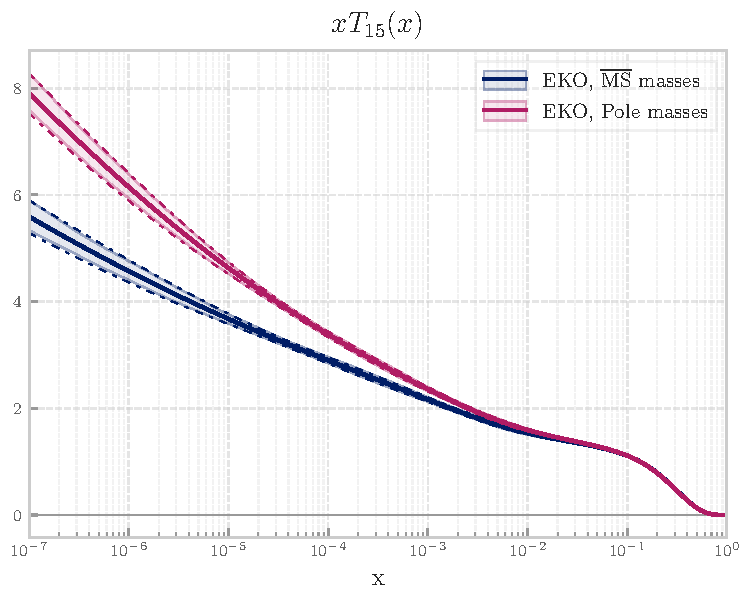
\includegraphics[width=0.47\linewidth]{ch-eko/msbar_T15.pdf}
    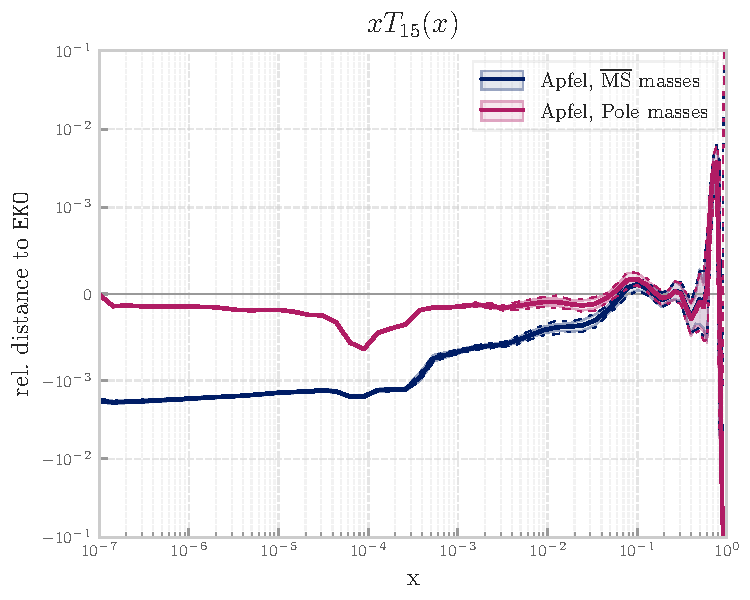
\includegraphics[width=0.47\linewidth]{ch-eko/msbar_bench_T15.pdf}
    \caption{(left) The NNPDF4.0 perturbative charm distribution
        $T_{15}(x)$~\cite{NNPDF:2021njg} with \msbar{} and pole masses \nnlo{}
        evolution when running on $\muF^2=\SI[parse-numbers=false]{1\to
        10^4}{\GeV^2}$.  (right) Relative difference to \eko{} for the same run
        with \apfel{}~\cite{Bertone:2013vaa}.}
     \label{fig:eko/MSbarbench}
\end{figure}

\begin{figure}
    \centering
    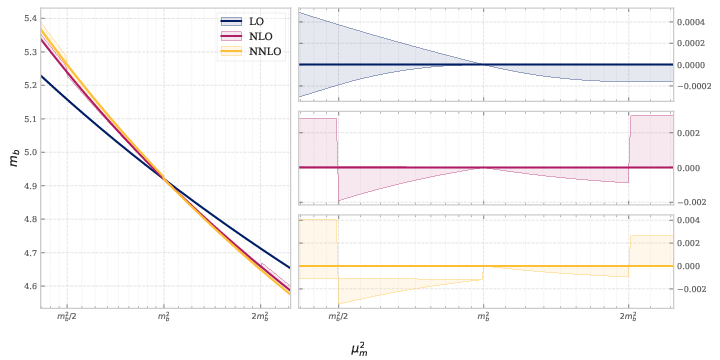
\includegraphics[width=\textwidth]{ch-eko/masses_running}
    \caption{Running of the bottom quark mass $m_b(\mu_m^2)$ for different threshold
        ratios, similar to \cref{fig:eko/asmatching}.
        The plot shows how the different choices of matching scales affect the
        running in the matching region (and slightly beyond) at \lo{}, \nlo{},
        and \nnlo{}.
        The border condition for the running has been chosen at $m_b(m_b) =
        \SI{4.92}{GeV}$, as it is clear from the plot, since it is the
        intersection point of all the curves shown.}
    \label{fig:eko/runningmasses}
\end{figure}


In \cref{fig:eko/runningmasses} we show the evolution of the \msbar{} bottom mass
$m_b(\mu_m^2)$ using different matching scales $\mu_b^2$ equal to $1/2,1$ and
$2$ times the mass $m_b^2$, for each perturbative order (\lo{}, \nlo{}, and
\nnlo{}).
The curve for $\mu_b^2 = m_b^2$ has been plotted as the central one (bold),
while the other two are used as the upper and lower borders of the shaded area
(according to their value, point by point).
The reference value $m_b(\mu_{b,0}^2)$, has been chosen equal for the
three curves, and it has been chosen at $m_b(m_b) = \SI{4.92}{GeV}$.
For this reason, above the central matching point $\mu_m^2 \ge m_b^2$ two curves coincide
($\mu_b^2 = m_b^2$ and $\mu_b^2 = m_b^2/2$) since they are both
running with the same number of flavors ($n_f=5$) and they have the same
border condition. The curve using $\mu_b^2 = 2m_b^2$, however, still runs with
a smaller number of flavors ($n_f=4$) and so does not match the former two.
In the lower region $\mu_m^2 < m_b^2$ this is not happening, because even
if the number of flavors is now the same,
the border condition is specified above matching for $\mu_b^2 = m_b^2$ (in
$n_f=5$).
So, starting from $m_b^2$ and going downward, the central choice $\mu_b^2 =
m_b^2$ is matched first and then evolved, while the higher scale choice
$\mu_b^2 = 2m_b^2$ immediately runs with four light flavors at $m_b^2$. Thus
the difference consists just in the matching.
